We have made frequent references to \emph{glitches} in the detectors,
a type of noise consisting of short, transient features.  In
chapter~\ref{ch:search} we have also noted that such features in the
data can elevate $\rho(t)$ and produce spurious triggers.  We will
refer to triggers resulting from noise as \emph{background triggers}.

In order to claim the detection of a gravitational wave we must have a
candidate whose significance stands well above that of these
background triggers.  So far this thesis has focused on increasing the
efficiency of the search to increase the significance of the signals.
We now shift focus to reducing the number of triggers in the
background.  The key to doing this is ability to \emph{veto} time,
that is, remove from the analysis times which we believe will
contribute excessively to the background and/or times in which we
would be unable to confidently detect a real signal.

In this chapter we discuss the infrastructure that enables such
vetoes.  In the next chapter we look at a tool, \emph{daily ihope},
which was used in S6 to characterize the behavior of the detectors and
determine times that needed to be vetoed.


\section{Data Quality Flags}
\label{sec:dq_flags}

The LIGO and Virgo detectors are extremely sophisticated, complex, and
sensitive.  Glitches can be produced in and by many parts of the
detector, and may ultimately be caused by either environmental
conditions or conditions internal to the detectors.  A great deal of
information about the state of the detector is recorded in
\emph{channels}, which are time series sampled from 1 Hz to 16 kHz,
depending on the channel.  These include such information as
\begin{itemize}
\item the power at which the Laser is operating
\item the output of every photodiode throughout the detector
\item the power in seismic noise in various frequency bands
\item the activity of the control servos
\end{itemize}
%
and a great deal more.  When any of these exceed normal operating
values it may indicate the presence of glitches, or even be their root
cause.  It is therefore extremely valuable to both data analysts and 
commissioners working on the detector to be able to \emph{flag} any
anomalous conditions.

The first line of defense against glitches is on-site as the
detector is running.  At all such times the control room is staffed
by an operator, an employee of LIGO labs who is an expert in running
the detector, and a science monitor
(``SciMon'') who is a member of the LIGO Scientific Collaboration
(LSC).  Either may flag times of unusual activity such as

\begin{itemize}
\item movement of heavy machinery on the site 
\item nearby storms 
\item modification of control parameters 
\end{itemize}
%
The operator and SciMon also jointly decide when to flag time as
suitable for analysis.  This depends on a few conditions; there must
be laser light in both arms and the detector must be \emph{locked},
meaning the cavities are on resonance.  When such conditions are met
the operator and SciMon can choose to enable \emph{science mode}.  Any
time such flagged will be included in the LIGO searches.

In addition to such manually-created flags, flags may be created
automatically by scanning the channel data.  This is done by a program
called the \emph{Data Monitoring Tool} (DMT) which records conditions
such as
%
\begin{itemize}
\item an instrumental channel has exceeded a threshold
\item the standard deviation of a channel has exceeded its expected
value
\item elevated seismic noise in a frequency band
\item the detector is properly locked
\end{itemize}
%
Note that these are all yes-or-no conditions.  Flags do not store
values, such as the level of seismic noise.  That information is
available in the channel data, the flags are intended to provide the
simplest possible summary of conditions.  At any given time a flag can
be in any of three states: on, off, or undefined.  Flags are undefined
during times when the responsible DMT process was not running.

In order to be useful flags must be represented in a standard format
and accessible to members of the LSC.  We start by identifying a flag
as a triple of (detector id, flag name, version number).
\emph{detector id} identifies the detector with a two-letter
abbreviation; H1, L1, V1 for Hanford, Livingston and Virgo
respectively.  \emph{flag name} is a unique identifier, to prevent
confusion with case sensitivity in processing tools, all DQ flag names
were required to be in upper case case. Additionally, a 3-letter
prefix was be added to each flag name to better identify the source
where data came from. For example: the flag indicating high wind speed
would be \texttt{DMT-WIND\_OVER\_30MPH}.  \emph{version number} is an
integer starting from 1.  Version numbers can change if, for example,
a bug is found in one of the DMT processes.  Once the bug is fixed the
DMT can be rerun over the original channel data to produce the next
subsequent version of the flag.  However, by storing all prior
versions we are able to reconstruct the results of earlier searches. 

Conceptually, managing flag information consists of providing
functions that
%
\begin{itemize}
\item map from a flag (ifo id, flag name, version number) to a set of
times where the flag was defined
\item map from a flag (ifo id, flag name, version number) to a set of
times where the flag was active
\end{itemize}
%
The times
during which the flag was inactive, if needed, can be obtained from the
difference between these two.  It is also useful to think of these
functions as mapping (ifo id, flag name, version number, time) to an
``active, inactive or undefined'' indicator, or mapping a time to a
set of flags that are active.


% https://www.lsc-group.phys.uwm.edu/daswg/wiki/content_of_segment_publication_and_discovery



%%%%%%%%%%%%%%%%%%%%%%%%%%%%%%%%%

\section{Implementation Details}

The implementation of the maps between flags and sets of times is
conceptually straightforward.  We represent sets of times as sets of
\emph{segments}, which are half-open intervals aligned on GPS-second
boundaries.  We can assign to each flag triple a unique integer
identifier, and then store segments as triples of (id, start time, end
time).  The functions above then consist of looking up the flag,
determining the identifier, then returning all segments with matching
identifiers.  We will need two such segment stores, one for
``defined'' segments and one for ``active'' segments.  We will call
the map between flags and identifiers the \texttt{segment\_definer},
the store of ``defined'' segments will be called the
\texttt{segment\_summary}, and we we reserve the name \texttt{segment}
for the store of active segments.

We now have a structure in which data quality flags can be stored.
In S6 this was implemented in two ways:
%
\begin{enumerate}
\item as files in eXtensible Markup Language (XML) format.  XML is a
scheme for adding structure to documents~\cite{xmlconsortium}.  It is
relatively simple in that XML files can be read and modified by
standard text editors.  The LSC utilizes a specialized form of XML
called \emph{LIGO light weight} or LIGO LW~\cite{LIGO-T990023-01}.
The names of most programs that produce or consume such files begin
with the prefix \texttt{ligolw\_}.  See
Sec.~\ref{sec:data_file_format} for more on this format.

\item in a relational database called the \emph{segment database},
hosted at CalTech.  This allowed high-speed, distributed
access to flag information.  See
Sec.~\ref{sec:segment_database_design} for more on the structure of
the database.
\end{enumerate}


\begin{figure}[h]
  \label{f:segment_flow}
  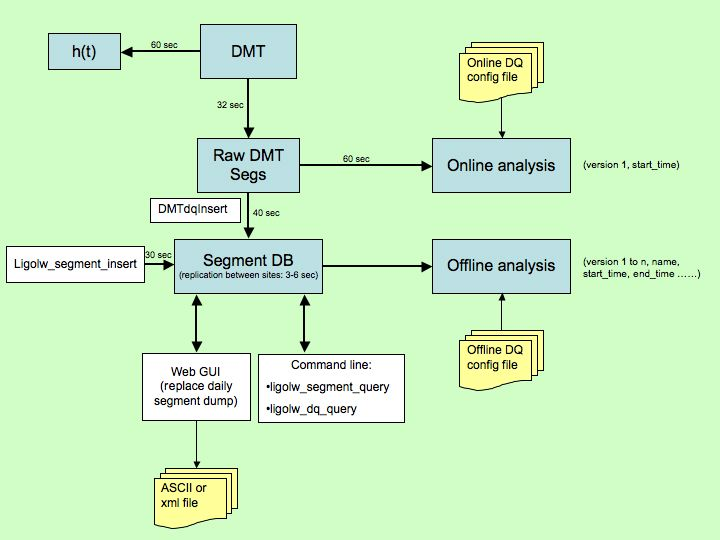
\includegraphics[width=\linewidth]{figures/segdb/T0900005_fig1}
  \caption[Flow of S6 data quality information]{
  Flow of S6 data quality segment information. Online data
  quality segments and science segment information is generated by the DMT.
  This can be directly queried for low-latency online analysis or inserted
  into a segment database for off-line or higher-latency analyses. Command
  line and web GUI tools were used to query and update the segment
  database.} 
\end{figure}

The flow of flag information is illustrated in
Fig.~\ref{f:segment_flow}:
%
\begin{enumerate}
\item \textbf{DMT} The DMT handled
the creation of all science segments and online data quality segments
in S6. Every 60 seconds, the DMT wrote segment
information in XML format to disk at each of the detectors. The DMT called
the \texttt{dmtdq\_seg\_insert} program to insert the XML data into
the segment database.

\item \textbf{Archival of DMT segment data:} The 60 second XML files
generated by the DMT were replicated to Caltech and other LSC
computing centers. Files were compressed using the gzip algorithm.

\item Software was developed to combine the segment
information from DMT XML files with a data quality categorization file
managed by the search groups (see Sec.~\ref{sec:veto_definer}
below) to produce files containing veto information for a given search
once per minute or so.  The same software was be made available for
interfacing with the segment database for offline searches and
detector characterization (see Sec.~\ref{ssec:from_cats}
below).

\item \textbf{Expected Latencies:} as described in the implementation plan
diagram, targeted latencies were:
\begin{itemize}
\item DMT generates h(t) file: 60 seconds
\item From DMT to raw DMT segment disk: 60 seconds
\item From raw DMT segment disk to segment database: 10 seconds
\item From ligolw\_segment\_insert to segment database: 30 seconds
\end{itemize}
\end{enumerate}



\section{Segment Data File Format}
\label{sec:data_file_format}

To be ingested into the segment database, segment data must be in the
format described in this section. Data should be in a valid LIGO LW
XML file with \verb|process|, \verb|segment_definer|,
\verb|segment_summary| and \verb|segment| tables. An optional
\verb|process_params| table can be used to store extra metadata about
segment generation.

The \verb|process| table should contain the columns given in the XML
file below which describe the name, version, cvs repository and
revision of the program used generate the data. The comment column can
be used to add additional human-readable data. The \verb|node|,
\verb|username|,
\verb|unix_procid|, \verb|start_time| and \verb|end_time| columns should store metadata
describing who ran the process and where it ran. The \verb|ifos| column
should contain an alphabetical list of all ifo data using as input to
the process. The \verb|process_id| column is used to link the defined
process to other rows in the file created by that process.

The \verb|segment_definer| table should contain a definition of the
segments included in the file. The \verb|ifos|, \verb|name| and
\verb|version| columns should contain the name and version of the
segment. The name should be upper case for all segments. DMT-derived
segments should be prefixed with the string \verb|DMT-|, segments
created by the detector characterization group should be prefixed with
\verb|DCH-| and segments from the Virgo database should be prefixed
with \verb|VDB-|.  The comment column can be used to add a
human-readable description of the segment. The \verb|segment_definer|
column is used to link this type of segment to the intervals in the
\verb|segment| and \verb|segment_summary| tables.

The \verb|segment| table should contain the GPS start and end time
when the segment described in the \verb|segment_definer| table was
\emph{active}. The \verb|segment_summary| table should contain the GPS
start time and end time of the interval for which the segment is
\emph{defined}. This will allow users to distinguish between the cases
where a DQ segment is undefined for a particular time or simply
inactive (i.e. it is \emph{not} windy, as opposed to the wind monitor
being down).

{\tiny
\begin{verbatim}
<?xml version="1.0"?>
<!DOCTYPE LIGO_LW SYSTEM "http://ldas-sw.ligo.caltech.edu/doc/ligolwAPI/html/ligolw_dtd.txt">
<LIGO_LW>
  <Table Name="processgroup:process:table">
    <Column Name="processgroup:process:program" Type="lstring"/>
    <Column Name="processgroup:process:version" Type="lstring"/>
    <Column Name="processgroup:process:cvs_repository" Type="lstring"/>
    <Column Name="processgroup:process:cvs_entry_time" Type="int_4s"/>
    <Column Name="processgroup:process:comment" Type="lstring"/>
    <Column Name="processgroup:process:node" Type="lstring"/>
    <Column Name="processgroup:process:username" Type="lstring"/>
    <Column Name="processgroup:process:unix_procid" Type="int_4s"/>
    <Column Name="processgroup:process:start_time" Type="int_4s"/>
    <Column Name="processgroup:process:end_time" Type="int_4s"/>
    <Column Name="processgroup:process:process_id" Type="ilwd:char"/>
    <Column Name="processgroup:process:ifos" Type="lstring"/>
    <Stream Name="processgroup:process:table" Type="Local" Delimiter=",">
      "SegGener","1.17",
      "/ldcg_server/common/repository_gds/gds/Monitors/SegGener/SegGener.cc\,v",
      865755895,"Segment generation from an OSC condition","granite","jzweizig",718,
      918756928,918836992,"process:process_id:0","H0H1H2"
    </Stream>
  </Table>
  <Table Name="segment_definergroup:segment_definer:table">
    <Column Name="segment_definergroup:segment_definer:process_id" Type="ilwd:char"/>
    <Column Name="segment_definergroup:segment_definer:segment_def_id" Type="ilwd:char"/>
    <Column Name="segment_definergroup:segment_definer:ifos" Type="lstring"/>
    <Column Name="segment_definergroup:segment_definer:name" Type="lstring"/>
    <Column Name="segment_definergroup:segment_definer:version" Type="int_4s"/>
    <Column Name="segment_definergroup:segment_definer:comment" Type="lstring"/>
    <Stream Name="segment_definergroup:segment_definer:table" Type="Local" Delimiter=",">
      "process:process_id:0","segment_definer:segment_def_id:35","H2","DMT-LIGHT",1,
      "H2 Light in arms from h(t) DQ flags",
      "process:process_id:0","segment_definer:segment_def_id:36","H2","DMT-SCIENCE",1,
      "H2 Science mode from h(t) DQ flags",
      "process:process_id:0","segment_definer:segment_def_id:37","H2","DMT-INJECTION",1,
      "H2 Injection mode from h(t) DQ flags",
      "process:process_id:0","segment_definer:segment_def_id:38","H2","DMT-UP",1,
      "H2 calibration OK in from h(t) DQ flags",
      "process:process_id:0","segment_definer:segment_def_id:39","H2","DMT-CALIBRATED",1,
      "H2 Calibration OK from h(t) DQ flags",
      "process:process_id:0","segment_definer:segment_def_id:40","H2","DMT-BADGAMMA",1,
      "H2 Bad gamma in h(t) DQ flags"
    </Stream>
  </Table>
  <Table Name="segmentgroup:segment:table">
    <Column Name="segmentgroup:segment:segment_id" Type="ilwd:char"/>
    <Column Name="segmentgroup:segment:start_time" Type="int_4s"/>
    <Column Name="segmentgroup:segment:end_time" Type="int_4s"/>
    <Column Name="segmentgroup:segment:segment_def_id" Type="ilwd:char"/>
    <Column Name="segmentgroup:segment:process_id" Type="ilwd:char"/>
    <Stream Name="segmentgroup:segment:table" Type="Local" Delimiter=",">
      "segment:segment_id:15",918836961,918836977,"segment_definer:segment_def_id:35",
      "process:process_id:0",
      "segment:segment_id:16",918836976,918836992,"segment_definer:segment_def_id:37",
      "process:process_id:0"
    </Stream>
  </Table>
  <Table Name="segment_summarygroup:segment_summary:table">
    <Column Name="segment_summarygroup:segment_summary:segment_sum_id" Type="ilwd:char"/>
    <Column Name="segment_summarygroup:segment_summary:start_time" Type="int_4s"/>
    <Column Name="segment_summarygroup:segment_summary:end_time" Type="int_4s"/>
    <Column Name="segment_summarygroup:segment_summary:comment" Type="lstring"/>
    <Column Name="segment_summarygroup:segment_summary:segment_def_id" Type="ilwd:char"/>
    <Column Name="segment_summarygroup:segment_summary:process_id" Type="ilwd:char"/>
    <Stream Name="segment_summarygroup:segment_summary:table" Type="Local" Delimiter=",">
      "segment_summary:segment_sum_id:5",918836976,918836992,"",
      "segment_definer:segment_def_id:40","process:process_id:0",
      "segment_summary:segment_sum_id:6",918836976,918836992,"",
      "segment_definer:segment_def_id:39","process:process_id:0",
      "segment_summary:segment_sum_id:11",918836976,918836992,"",
      "segment_definer:segment_def_id:37","process:process_id:0",
      "segment_summary:segment_sum_id:12",918836976,918836992,"",
      "segment_definer:segment_def_id:35","process:process_id:0",
      "segment_summary:segment_sum_id:42",918836976,918836992,"",
      "segment_definer:segment_def_id:36","process:process_id:0",
      "segment_summary:segment_sum_id:46",918836976,918836992,"",
      "segment_definer:segment_def_id:38","process:process_id:0"
    </Stream>
  </Table>
</LIGO_LW>
\end{verbatim}
}

%%%%%%%%%%%%%%%%%%%%%%%%%%%%%%%%%%%%%%%%%%%%%%%%
\section{S6 Segment Database Design}
\label{sec:segment_database_design}

The five tables used for the S6 segment database are shown in
Fig.~\ref{f:schema}.  Each table has a corresponding structure in
the XML files.  In addition to the \verb|segment_definer|,
\verb|segment_summary| and \verb|segment| tables discussed above, we
add \verb|process| and \verb|process_params| tables that indicate the
program that created each flag and how that program was run.

\begin{figure}[h]
  \begin{center}
    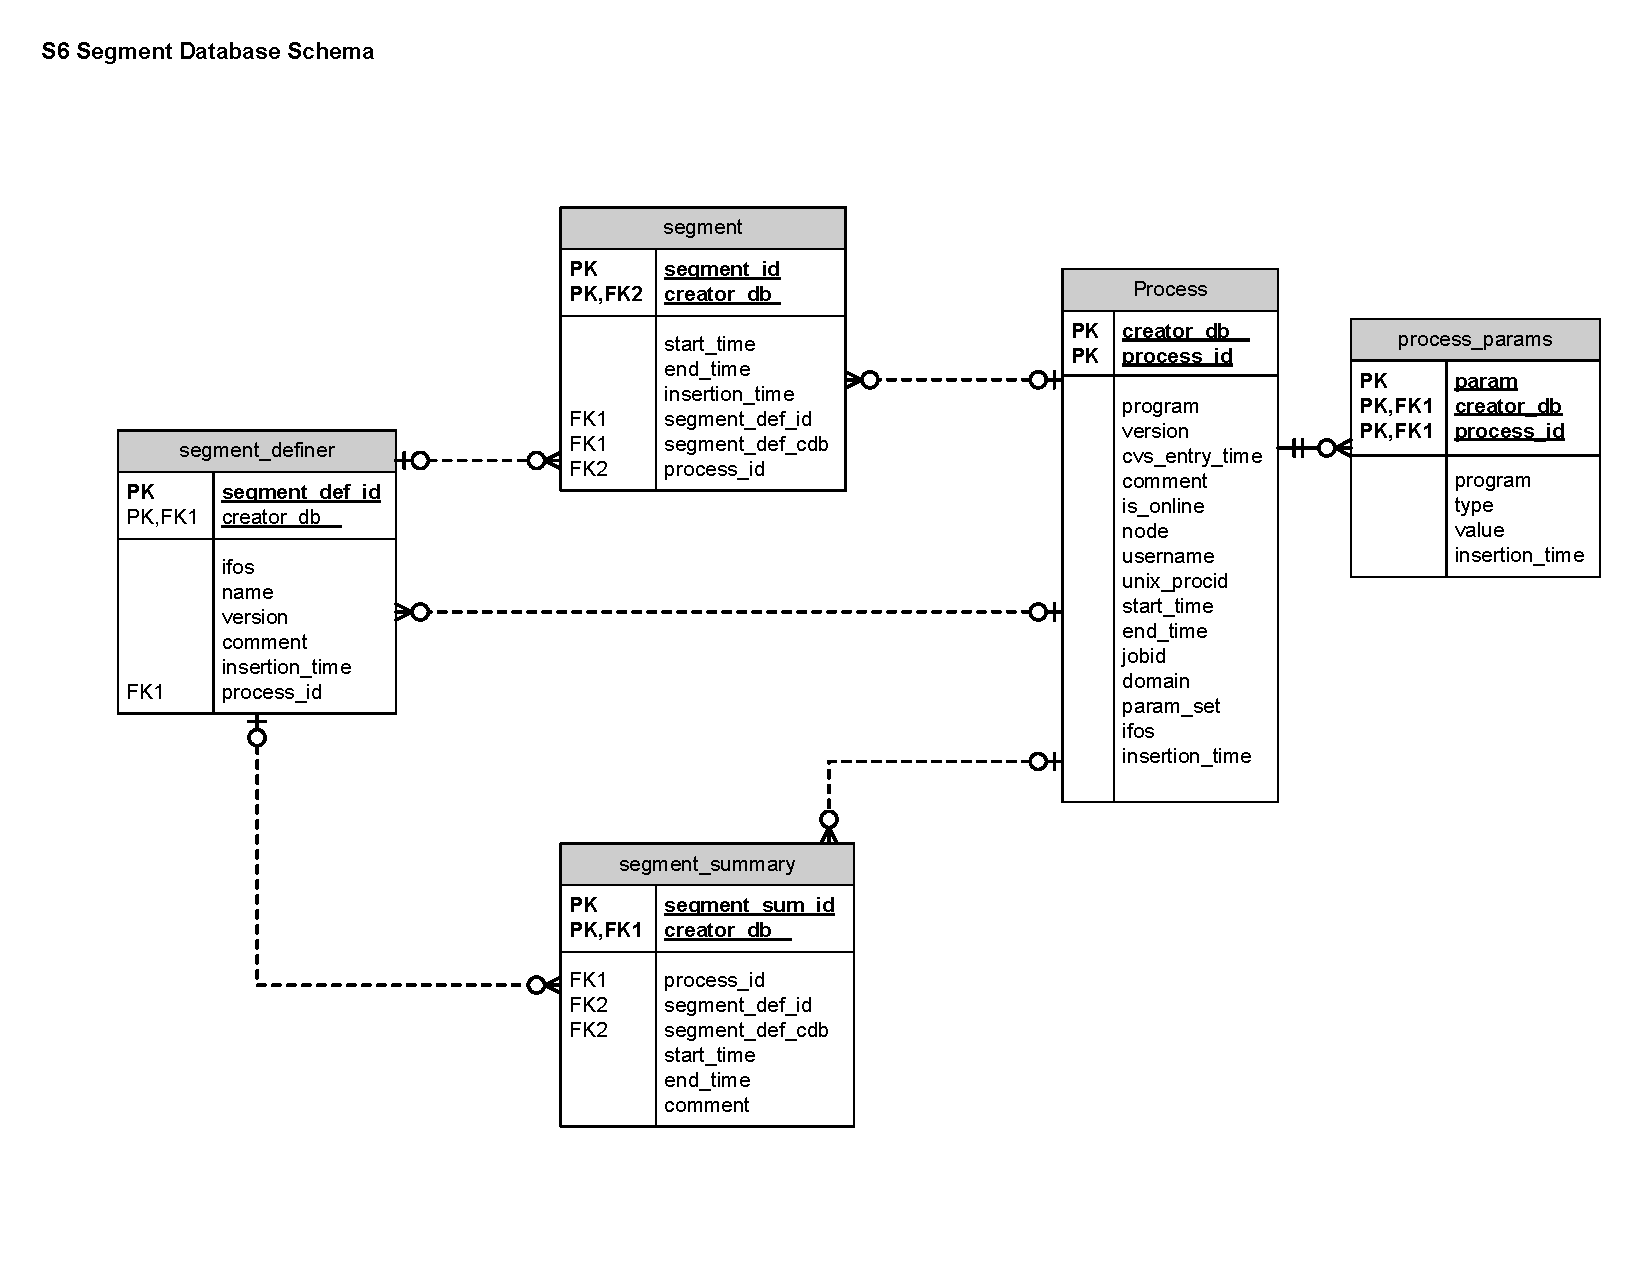
\includegraphics[width=0.9\linewidth]{figures/segdb/T0900005_fig3}
  \end{center}
  \label{f:schema}
  \caption[S6 Segment Database Scheme]{
Structure of the S6 segment database.  Each box represents a
\emph{table} (a set of structured data), the name of which is in grey.
The lines within the boxes are the names of \emph{columns}, individual
data elements within the table.  For example, the
\texttt{process\_params} table contains a set of \emph{rows}, each row
contains data elements named \texttt{program}, \texttt{type},
\texttt{value} and \texttt{intertion\_time}.

The lines between boxes indicate relations between tables.  For
example, the \texttt{segment\_definer} is connected to the
\texttt{segment\_summary} and \texttt{segment} tables through the 
\texttt{segment\_def\_id}.  This implements the conceptual relations
between these entities discussed above.
}
\end{figure}



%%%%%%%%%%%%%%%%%%%%%%%%%%%%%%%%%%%%%%%%%%%%%%%%%
\section{Command Line Tools}

We now turn to the tools that implemented the various mappings between
flags and sets of times discussed above.  Except where noted these
programs could all operate on either XML files or the segment
database.  Except for \texttt{ligolw\_segment\_insert} all programs
could only read information from the database, they could not add or
change existing data.  Flags were specified in the form
\texttt{ifo:name:version}.  For many programs the version could be
omitted and the program would report on the latest defined version.

\subsection{ligolw\_segment\_query}

\texttt{ligolw\_segment\_query} was designed to answer the following
questions:
%
\begin{itemize}
\item What DQ flags exist in the database?
\texttt{ligolw\_segment\_query --show-types}
\item When was a given flag inserted? \texttt{ligolw\_segment\_query
--query-types}
\item When was a given DQ flag defined? \texttt{ligolw\_segment\_query
--query-types}
\item When was a given flag active? \texttt{ligolw\_segment\_query
--query-segments}
\end{itemize}
%
The built-in help message, generated by \texttt{ligolw\_segment\_query
--help} is shown below:
%
{\small
\begin{verbatim}
DESCRIPTION:
  --version             show program's version number and exit
  -h, --help            show this help message and exit
  -p, --ping            Ping the target server
  -y, --show-types      Returns a xml table containing segment type
                        information: ifos, name, version,
                        segment_definer.comment, segment_summary.start_time,
                        segment_summary.end_time, segment_summary.comment
  -u, --query-types     Returns a ligolw document whose segment_definer table
                        includes all segment types defined in the given period
                        and included by include-segments and whose
                        segment_summary table indicates the times for which
                        those segments are defined.
  -q, --query-segments  Returns a ligolw document whose segment table contains
                        the times included by the include-segments flag and
                        excluded by exclude-segments
  -s gps_start_time, --gps-start-time=gps_start_time
                        Start of GPS time range
  -e gps_end_time, --gps-end-time=gps_end_time
                        End of GPS time range
  -t segment_url, --segment-url=segment_url
                        Segment URL. Users have to specify either 'https://'
                        for a secure connection or 'http://' for an insecure
                        connection in the segment database url. For example,
                        '--segment-url=https://segdb.ligo.caltech.edu'. No
                        need to specify port number.
  -d, --database        use database specified by environment variable
                        S6_SEGMENT_SERVER. For example,
                        'S6_SEGMENT_SERVER=https://segdb.ligo.caltech.edu'
  -f, --dmt-files       use files in directory specified by environment
                        variable ONLINEDQ, for example,
                        'ONLINEDQ=file:///path_to_dmt'. 'file://' is the
                        prefix, the acutal directory to DMT xml files starts
                        with '/'.
  -a include_segments, --include-segments=include_segments
                        This option expects a comma separated list of a colon
                        separated sublist of interferometer, segment type, and
                        version. The union of segments from all types and
                        versions specified is returned. Use --show-types to
                        see what types are available.   For example:
                        --include-segment-types H1:DMT-SCIENCE:1,H1:DMT-
                        INJECTION:2 will return the segments for which H1 is
                        in either SCIENCE version 1 or INJECTION version 2
                        mode. If version information is not provided, the
                        union of the segments of the latest version of
                        requested segment type(s) will be returned.
  -b exclude_segments, --exclude-segments=exclude_segments
                        This option has to be used in conjunction with
                        --include-segment-types --exclude-segment-types
                        subtracts the union of unwanted segments from the
                        specified types from the results of --include-segment-
                        types. If version information is not provided,
                        --exclude-segment-types subtracts the union of
                        segments from the latest version of the specified
                        segment types. For example, --include-segment-types H1
                        :DMT-SCIENCE:1,H1:DMT-INJECTION:2 --exclude-segment-
                        types H1:DMT-WIND:1,H1:DMT-NOT_LOCKED:2,H2:DMT-
                        NOT_LOCKED:2 will subtract the union of segments which
                        H1 is in version 1 WIND and H1,H2 is version 2
                        NOT_LOCKED from the result of --include-segment-types
                        H1:DMT-SCIENCE:1,H1:DMT-INJECTION:2
  -S, --strict-off      The default behavior is to truncate segments so that
                        returned segments are entirely in the interval [gps-
                        start-time, gps-end-time).  However if this option is
                        given, the entire non-truncated segment is returned if
                        any part of it overlaps the interval.
  -o output_file, --output-file=output_file
                        File to which output should be written.  Defaults to
                        stdout.
\end{verbatim}
}

\subsubsection{ligolw\_dq\_query}

Below are the questions that \texttt{ligolw\_dq\_query} was designed
to answer:
%
\begin{itemize}
\item is a given flag active at a given time?
\texttt{ligolw\_dq\_query --active}
\item is a given flag defined at a given time?
\texttt{ligolw\_dq\_query --defined}
\item what is the status of all flags at a given time?
\texttt{ligolw\_dq\_query --report}
\end{itemize}
%
The built-in help message, generated by \texttt{ligolw\_dq\_query
--help} is shown below:
%
{\small
\begin{verbatim}
DESCRIPTION:
  --version             show program's version number and exit
  -h, --help            show this help message and exit
  -p, --ping            Ping the target server
  -y, --defined         Returns a segment summary table containing segments
                        defined at the given time(s).
  -u, --active          Returns a segment table containing segments active at
                        the given time(s).
  -q, --report          Prints which flags are defined/undefined at the given
                        time(s). For the flags which were defined, it
                        determines if the flag was active or inactive at that
                        time. For an active flag, it prints the start and end
                        time of the segment to which the active. For an
                        inactive flag, it prints the end time of the previous
                        adjacent active segment and the start time of the next
                        adjacent active segment
  -s start_pad, --start-pad=start_pad
                        Seconds before given time(s) to include in query
  -e end_pad, --end-pad=end_pad
                        Seconds after given time(s) to include in query
  -t segment_url, --segment-url=segment_url
                        Segment URL
  -d, --database        use database specified by environment variable
                        S6_SEGMENT_SERVER
  -f, --dmt-files       use files in directory specified by environment
                        variable ONLINEDQ
  -a include_segments, --include-segments=include_segments
                        This option expects a comma separated list of a colon
                        separated sublist of interferometer, segment type, and
                        version. The union of segments from all types and
                        versions specified is returned. Use --show-types to
                        see what types are available.   For example:
                        --include-segment-types H1:SCIENCE:1,H1:INJECTION:2
                        will return the segments for which H1 is in either
                        SCIENCE version 1 or INJECTION version 2 mode. If
                        version information is not provided, the union of the
                        segments of the latest version of requested segment
                        type(s) will be returned.
  -o output_file, --output-file=output_file
                        File to which output should be written.  Defaults to
                        stdout.
  -i, --in-segments-only
                        If set, report will only return segments that given
                        times were within
\end{verbatim}
}



\subsubsection{ligolw\_segments\_from\_cats}
\label{ssec:from_cats}

\texttt{ligolw\_segments\_from\_cats} read a veto definer file (see
Sec.~\ref{sec:veto_definer}) and accessed either segment XML files
or the segment database in order to produce a list of times to be
vetoed.  The built-in help message is displayed below:
%
{\small
\begin{verbatim}
DESCRIPTION:
  --version             show program's version number and exit
  -h, --help            show this help message and exit
  -v veto_file, --veto-file=veto_file
                        veto XML file (required).
  -o output_dir, --output-dir=output_dir
                        Directory to write output (default=cwd).
  -k, --keep-db         Keep sqlite database.
  -t segment_url, --segment-url=segment_url
                        Segment URL
  -d, --database        use database specified by environment variable
                        S6_SEGMENT_SERVER
  -f, --dmt-file        use files in directory specified by environment
                        variable ONLINEDQ
  -c, --cumulative-categories
                        If set the category N files will contain all segments
                        in categories <= N
  -p, --separate-categories
                        If set the category N files will contain only category
                        N
  -s gps_start_time, --gps-start-time=gps_start_time
                        Start of GPS time range
  -e gps_end_time, --gps-end-time=gps_end_time
                        End of GPS time range
\end{verbatim}
}

For example:
\begin{alltt}
ligolw\_segments\_from\_cats
  --gps-start-time 930960015
  --gps-end-time 931564887
  --segment-url https://segdb.ligo.caltech.edu:30015
  --cumulative-categories
  --veto-file H1L1V1-S6\_CBC\_LOWMASS\_ONLINE-928271454-0.xml
\end{alltt}




\subsubsection{ligolw\_segment\_insert}

\texttt{ligolw\_segment\_insert} handled two tasks:
%
\begin{itemize}
\item Insert segments and/or segment types into the segment database.
\item Append segments to the existing segment types.
\end{itemize}
%
This program uses the terminology IFO (\emph{Interferometric Observatory})
instead of ``detector.''  The built-in help message is displayed below:
%
{\small
\begin{verbatim}
DESCRIPTION:
  -h, --help            show this help message and exit
  -p, --ping            Ping the target server
  -t URL, --segment-url=URL
                        Users have to specify protocol 'https://' for a secure
                        connection in the segment database url. For example,
                        '--segment-url=https://segdb.ligo.caltech.edu'. No
                        need to specify port number'.
  -o FILE, --output=FILE
                        Write segments to FILE rather than the segment
                        database
  -j IDENTITY, --identity=IDENTITY
                        Set the subject line of the server's service
                        certificate to IDENTITY
  -I, --insert          Insert segments to the segment database
  -A, --append          Append segments to an existing segment type
  -i IFOS, --ifos=IFOS  Set the segment interferometer to IFOS (e.g. H1)
  -n NAME, --name=NAME  Set the name of the segment to NAME (e.g. DMT-
                        BADMONTH)
  -v VERSION, --version=VERSION
                        Set the numeric version of the segment to VERSION
                        (e.g. 1)
  -e EXPLAIN, --explain=EXPLAIN
                        Set the segment_definer:comment to COMMENT. This
                        should explaining WHAT this flag mean (e.g. "Light dip
                        10%"). Required when --Insert/-I is specified.
  -c COMMENT, --comment=COMMENT
                        Set the segment_summary:comment to COMMENT. This
                        should explaining WHY these segments were inserted
                        (e.g. "Created from hveto results")
  -S FILE, --summary-file=FILE
                        Read the segment_summary rows from FILE. This should
                        be a file containing the gps start and end times that
                        the flag was defined, deliminated by comma (i.e. the union of on and off)
  -G FILE, --segment-file=FILE
                        Read the segment rows from FILE. This should containin
                        the gps start and end times when the flag was active deliminated by comma
\end{verbatim}
%
As an example, the command to insert segments of a new type would 
look like:
%
\begin{alltt}
ligolw\_segment\_insert
  --segment-url https://segdb.ligo.caltech.edu
  --ifos 'H1'
  --name 'DCH-TEST'
  --version 1
  --comment 'testing if insert works'
  --explain 'test insert'
  --segment-file segment.txt
  --summary-file summary.txt
  --insert
\end{alltt}

To append segments to an existing segment, the command would look like:
%
\begin{alltt}
ligolw\_segment\_insert 
  --segment-url https://segdb.ligo.caltech.edu
  --ifos 'H1'
  --name 'DCH-TEST'
  --version 1
  --comment 'testing if append works'
  --segment-file append\_segment.txt
  --summary-file append\_summary.txt
  --append
\end{alltt}


\subsection{The Veto Definer}
\label{sec:veto_definer}

Problems in the data may have differing levels of severity, and
consequently we define several \emph{veto categories} to characterize
them.  We defer discussion of the meaning of these categories until
the next chapter, but note here that the categories are indicated by
integers from 1 to 4, in decreasing levels of severity.  These
categories are commonly referred to as \emph{CAT1} through
\emph{CAT4}.  We also note that time marked with CAT1 is
entirely excluded form the analysis.  4091 seconds of data with one
second of CAT1 time in the middle will be split into two
2045-second chunks.  Neither of these will be analyzable by the ihope
pipeline, which requires 2048 seconds of data in order to compute the
PSD as discussed in Sec.~\ref{sec:search_pipeline}.  Short CAT1
vetos can therefore effectively veto much larger times, and such
vetoes are therefore to be avoided whenever possible. 

In order to veto a chunk of time it is necessary to map a data quality
flag to a veto category.  This is accomplished with a \emph{veto
definer file}.  Such files are specific to each search, as time that
is problematic for one search may pose no issues for another.  The
\texttt{ligolw\_segments\_from\_cats} program (see above) merges the
information in this file with the set of active flag segments to
produce \emph{veto segments} at each veto level.  Analysis is
performed on times marked as science with no CAT1 vetoes.  Triggers
from times marked as CAT2, CAT3 and CAT4 are discarded from both
foreground and background.

In some circumstances the search is more sensitive to anomalous
conditions than the DMT and excess triggers may be produced outside
the time covered by the flag.  This is one motivation for using the
search itself as a data quality tool, as discussed in the next
chapter.  The veto definer file therefore allows for \emph{padding},
offsets which effectively extend the flags.  The padding used will be
specific to each search, as different searches will be sensitive to
different classes of problems over different extents.

\subsection{Example Veto Configuration File}

The veto configuration file should contain a \verb|process| table
describing how it was created and a \verb|veto_definer| table
describing the flags to be applied at different levels. The comment
column of the process table should contain the version of the file.
The columns in the \verb|veto_definer| table are as follows:
\verb|ifo|, \verb|name| and \verb|version| uniquely define a
particular DQ/veto flag. \verb|category| indicates at which category
the veto should be applied, \verb|start_time|
and \verb|end_time| denote the GPS time interval for which the DQ/veto
flag should be applied (Note: if \verb|end_time| is zero, then the
current GPS time is assumed). \verb|start_pad| and \verb|end_pad| are
the padding time (in seconds) applied to the start and end of the veto
segments. Note that these are signed: if you want time vetoed to start
time to be \emph{earlier} than the start time listed in the database,
then the emph \verb|start_pad| should be \emph{negative}. Similarly,
if the time vetoed should extend \emph{after} the end time stored in
the database, then the value in \verb|end_pad| should be
\emph{positive}. The \verb|comment| column can be used to store an
optional human-readable comment.

{\tiny
\begin{verbatim}
<?xml version='1.0' encoding='utf-8' ?>
<!DOCTYPE LIGO_LW SYSTEM "http://ldas-sw.ligo.caltech.edu/doc/ligolwAPI/html/ligolw_dtd.txt">
<LIGO_LW>
   <Table Name="process:table">
      <Column Name="process:process_id" Type="ilwd:char"/>
      <Column Name="process:program" Type="lstring"/>
      <Column Name="process:version" Type="lstring"/>
      <Column Name="process:cvs_repository" Type="lstring"/>
      <Column Name="process:cvs_entry_time" Type="int_4s"/>
      <Column Name="process:node" Type="lstring"/>
      <Column Name="process:username" Type="lstring"/>
      <Column Name="process:unix_procid" Type="int_4s"/>
      <Column Name="process:start_time" Type="int_4s"/>
      <Column Name="process:end_time" Type="int_4s"/>
      <Column Name="process:ifos" Type="lstring"/>
      <Column Name="process:comment" Type="lstring"/>
      <Stream Name="process:table" Type="Local" Delimiter=",">
      "process:process_id:0","ligolw_veto_file","1.1",
      "/usr/local/cvs/lscsoft/glue/bin/ligolw_veto_file,v",822908378,
      "ldas-grid.ligo.caltech.edu","jrsmith",16830,822879594,822879594,
      "H1","Example file by Josh"
      </Stream>
   </Table>
   <Table Name="veto_definer:table">
      <Column Name="veto_definer:process_id" Type="ilwd:char"/>
      <Column Name="veto_definer:ifo" Type="lstring"/>
      <Column Name="veto_definer:name" Type="lstring"/>
      <Column Name="veto_definer:version" Type="int_4s"/>
      <Column Name="veto_definer:category" Type="int_4s"/>
      <Column Name="veto_definer:start_time" Type="int_4s"/>
      <Column Name="veto_definer:end_time" Type="int_4s"/>
      <Column Name="veto_definer:start_pad" Type="int_4s"/>
      <Column Name="veto_definer:end_pad" Type="int_4s"/>
      <Column Name="veto_definer:comment" Type="lstring"/>
      <Stream Name="veto_definer:table" Type="Local" Delimiter=",">
      "process:process_id:0","H1","OUT_OF_LOCK",0,1,917985615,0,0,0,"",
      "process:process_id:0","H1","BADGAMMA",1,1,917985615,0,0,0,"",
      "process:process_id:0","H1","ASC_Overflow",0,2,917985615,0,-8,8,"ASC saturations are cat2",
      "process:process_id:0","H1","PD_Overflow",0,2,917985615,0,-8,8,"PD saturations are cat2",
      "process:process_id:0","H1","SEVERE_LSC_OVERFLOW",0,2,917985615,0,-8,8,"LSC saturations are cat2",
      "process:process_id:0","H1","INJECTION",1,2,917985615,0,-16,64,"Remove HW injections at cat1",
      "process:process_id:0","H1","ASC_Overflow",0,3,917985615,0,-8,25,"ASC saturations are cat3 with larger pad",
      "process:process_id:0","H1","SEVERE_LSC_OVERFLOW",0,3,917985615,0,-8,25,"LSC saturations are cat3 with larger pad",
      "process:process_id:0","H1","PD_Overflow",0,3,917985615,0,-8,25,"PD saturations are cat3 with larger pad",
      "process:process_id:0","H1","Wind_over_30MPH",0,3,917985615,0,-8,8,"Windy",
      "process:process_id:0","H1","LIGHTDIP_1_PERCENT",0,3,917985615,0,-2,2,"Exclude all lightdip segments",
      "process:process_id:0","H1","PRE_LOCKLOSS_10_SEC",0,3,917985615,0,0,0,"",
      "process:process_id:0","H1","PRE_LOCKLOSS_30_SEC",0,3,917985615,0,0,0,"",
      "process:process_id:0","H1","PRE_LOCKLOSS_60_SEC",0,3,917985615,0,0,0,"",
      "process:process_id:0","H1","PRE_LOCKLOSS_120_SEC",0,3,917985615,0,0,0,"",
      "process:process_id:0","H1","ASI_CORR_OVERFLOW",0,4,917985615,0,-8,25,"Does this make sense for DC readout",
      "process:process_id:0","H1","LSC_OVERFLOW",0,4,917985615,0,-8,25,"LSC saturations",
      "process:process_id:0","H1","PRE_LOCKLOSS_600_SEC",0,4,917985615,0,0,0,"",
      "process:process_id:0","H1","PRE_LOCKLOSS_1800_SEC",0,4,917985615,0,0,0,""
      </Stream>
   </Table>
</LIGO_LW>
\end{verbatim}
}


